
\begin{par}
\section{ Kernel function }
\end{par} \vspace{1em}
\begin{par}
Gradient matching with Gaussian processes assumes a joint Gaussian process prior on states and their derivatives:
\end{par} \vspace{1em}
\begin{par}
$\left(\begin{array}{c} \mathbf{X} \\ \dot{\mathbf{X}} \end{array}\right)  \sim \mathcal{N} \left( \begin{array}{c} \mathbf{X} \\ \dot{\mathbf{X}} \end{array}; \begin{array}{c}  \mathbf{0} \\ \mathbf{0}  \end{array}, \begin{array}{cc}  \mathbf{C}_{\phi} & \mathbf{C}_{\phi}' \\ '\mathbf{C}_{\phi} &  \mathbf{C}_{\phi}'' \end{array} \right)$,
\end{par} \vspace{1em}
\begin{par}
$\mathrm{cov}(x_k(t), x_k(t)) = C_{\phi_k}(t,t')$
\end{par} \vspace{1em}
\begin{par}
$\mathrm{cov}(\dot{x}_k(t), x_k(t)) = \frac{\partial C_{\phi_k}(t,t') }{\partial t} =: C_{\phi_k}'(t,t')$
\end{par} \vspace{1em}
\begin{par}
$\mathrm{cov}(x_k(t), \dot{x}_k(t)) = \frac{\partial C_{\phi_k}(t,t') }{\partial t'} =: {'C_{\phi_k}(t,t')}$
\end{par} \vspace{1em}
\begin{par}
$\mathrm{cov}(\dot{x}_k(t), \dot{x}_k(t)) = \frac{\partial C_{\phi_k}(t,t') }{\partial t \partial t'} =: C_{\phi_k}''(t,t')$.
\end{par} \vspace{1em}
\color{RoyalPurple}\begin{verbatim}
function [dC_times_invC,inv_C,A_plus_gamma_inv] = kernel_function(kernel,state,time_est)
\end{verbatim}
\color{black}
\color{RoyalPurple}\begin{verbatim}
kernel.param_sym = sym('rbf_param%d',[1,2]); assume(kernel.param_sym,'real');
kernel.t1 = sym('time1'); assume(kernel.t1,'real'); kernel.t2 = sym('time2');
assume(kernel.t2,'real');
\end{verbatim}
\color{black}

RBF kernel
\color{RoyalPurple}\begin{verbatim}
kernel.func = kernel.param_sym(1).*exp(-(kernel.t1-kernel.t2).^2./...
    (kernel.param_sym(2).^2));
kernel.name = 'rbf';
\end{verbatim}
\color{black}
\begin{par}
kernel derivatives
\end{par} \vspace{1em}
\color{RoyalPurple}\begin{verbatim}
for i = 1:length(kernel)
    kernel.func_d = diff(kernel.func,kernel.t1);
    kernel.func_dd = diff(kernel.func_d,kernel.t2);
    GP.fun = matlabFunction(kernel.func,'Vars',{kernel.t1,kernel.t2,kernel.param_sym});
    GP.fun_d = matlabFunction(kernel.func_d,'Vars',{kernel.t1,kernel.t2,kernel.param_sym});
    GP.fun_dd = matlabFunction(kernel.func_dd,'Vars',{kernel.t1,kernel.t2,...
        kernel.param_sym});
end
\end{verbatim}
\color{black}
\begin{par}
populate GP prior covariance matrix
\end{par} \vspace{1em}
\color{RoyalPurple}\begin{verbatim}
for t=1:length(time_est)
    C(t,:)=GP.fun(time_est(t),time_est,kernel.param);
    dC(t,:)=GP.fun_d(time_est(t),time_est,kernel.param);
    Cd(t,:)=GP.fun_d(time_est,time_est(t),kernel.param);
    ddC(t,:)=GP.fun_dd(time_est(t),time_est,kernel.param);
end
\end{verbatim}
\color{black}
\begin{par}
check GP prior covariance scaling
\end{par} \vspace{1em}
\color{RoyalPurple}\begin{verbatim}
[~,D] = eig(C); perturb = abs(max(diag(D))-min(diag(D))) / 10000;
if any(diag(D)<1e-6)
    C(logical(eye(size(C,1)))) = C(logical(eye(size(C,1)))) + perturb.*rand(size(C,1),1);
end
[~,D] = eig(C);
if any(diag(D)<0)
    error('C has negative eigenvalues!');
elseif any(diag(D)<1e-6)
    warning('C is badly scaled');
end
inv_C = inv_chol(chol(C,'lower'));

dC_times_invC = dC * inv_C;
\end{verbatim}
\color{black}
\begin{par}
plot samples from GP prior
\end{par} \vspace{1em}
\color{RoyalPurple}\begin{verbatim}
figure(3);
hold on; plot(time_est,mvnrnd(zeros(1,length(time_est)),C(:,:,1),3),'LineWidth',2);
h1 = gca; h1.FontSize = 20; h1.XLabel.String = 'time'; h1.YLabel.String = 'state value';
h1.Title.String = [kernel.name ' kernel'];
\end{verbatim}
\color{black}

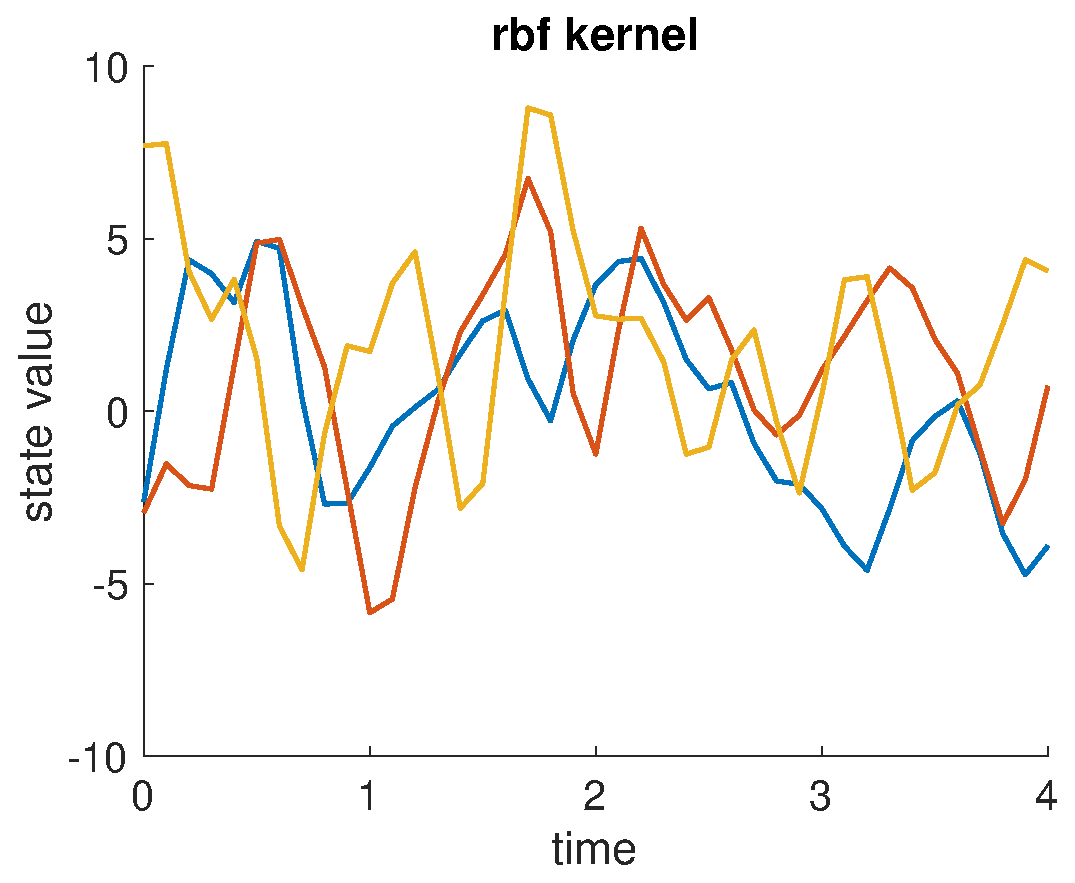
\includegraphics [width=5in]{Lotka_Volterra_3_04.eps}
\begin{par}
determine $(\mathbf{A} + \mathbf{I}\gamma)^{-1}$:
\end{par} \vspace{1em}
\color{RoyalPurple}\begin{verbatim}
A = ddC - dC_times_invC * Cd;
A_plus_gamma = A + state.derivative_variance(1) .* eye(size(A));
A_plus_gamma = 0.5.*(A_plus_gamma+A_plus_gamma');  % ensure that A plus gamma is symmetric
A_plus_gamma_inv = inv_chol(chol(A_plus_gamma,'lower'));
\end{verbatim}
\color{black}
\color{RoyalPurple}\begin{verbatim}
end
\end{verbatim}
\color{black}
\begin{par}
\section{ Fitting state observations }
\end{par} \vspace{1em}
\begin{par}
We fit the observations of state trajectories by standard GP regression.
\end{par} \vspace{1em}
\begin{par}
$p(\mathbf{X} \mid \mathbf{Y}, \phi,\gamma) = \prod_k \mathcal{N}(\mathbf{x}_k ; \boldmath\mu_k(\mathbf{y}_k),\boldmath\Sigma_k)$,
\end{par} \vspace{1em}
\begin{par}
where $\boldmath\mu_k(\mathbf{y}_k) := \sigma_k^{-2} \left(\sigma_k^{-2} \mathbf{I} + \mathbf{C}_{\boldmath\phi_k}^{-1} \right)^{-1} \mathbf{y}_k$ and $\boldmath\Sigma_k ^{-1}:=\sigma_k^{-2} \mathbf{I} + \mathbf{C}_{\boldmath\phi_k}^{-1}$.
\end{par} \vspace{1em}
\color{RoyalPurple}\begin{verbatim}
function [mu_u,inv_sigma_u,state] = fitting_state_observations(state,inv_C,...
    obs_to_state_relation,simulation)
\end{verbatim}
\color{black}
\begin{par}
Dimensions
\end{par} \vspace{1em}
\color{RoyalPurple}\begin{verbatim}
numb_states = size(state.sym.mean,2);
numb_time_points = size(state.sym.mean,1);
\end{verbatim}
\color{black}
\begin{par}
Variance of state observations
\end{par} \vspace{1em}
\color{RoyalPurple}\begin{verbatim}
state_obs_variance = simulation.state_obs_variance(state.obs);
\end{verbatim}
\color{black}
\begin{par}
Form block-diagonal matrix out of $\mathbf{C}_{\boldmath\phi_k}^{-1}$
\end{par} \vspace{1em}
\color{RoyalPurple}\begin{verbatim}
inv_C_replicas = num2cell(inv_C(:,:,ones(1,numb_states)),[1,2]);
inv_C_blkdiag = sparse(blkdiag(inv_C_replicas{:}));
\end{verbatim}
\color{black}
\begin{par}
GP posterior inverse covariance matrix: $\boldmath\Sigma_k ^{-1}:=\sigma_k^{-2} \mathbf{I} + \mathbf{C}_{\boldmath\phi_k}^{-1}$
\end{par} \vspace{1em}
\color{RoyalPurple}\begin{verbatim}
dim = size(state_obs_variance,1)*size(state_obs_variance,2);
% covariance matrix of error term (big E):
D = spdiags(reshape(state_obs_variance.^(-1),[],1),0,dim,dim) * speye(dim);
A_times_D_times_A = obs_to_state_relation' * D * obs_to_state_relation;
inv_sigma = A_times_D_times_A + inv_C_blkdiag;
\end{verbatim}
\color{black}
\begin{par}
GP posterior mean: $\boldmath\mu_k(\mathbf{y}_k) := \sigma_k^{-2} \left(\sigma_k^{-2} \mathbf{I} + \mathbf{C}_{\boldmath\phi_k}^{-1} \right)^{-1} \mathbf{y}_k$
\end{par} \vspace{1em}
\color{RoyalPurple}\begin{verbatim}
mu = inv_sigma \ obs_to_state_relation' * D * reshape(state.obs,[],1);
\end{verbatim}
\color{black}
\begin{par}
Reshape GP mean
\end{par} \vspace{1em}
\color{RoyalPurple}\begin{verbatim}
mu_u = zeros(numb_time_points,numb_states);
for u = 1:numb_states
    idx = (u-1)*numb_time_points+1:(u-1)*numb_time_points+numb_time_points;
    mu_u(:,u) = mu(idx);
end
\end{verbatim}
\color{black}
\begin{par}
Reshape GP inverse covariance matrix
\end{par} \vspace{1em}
\color{RoyalPurple}\begin{verbatim}
inv_sigma_u = zeros(numb_time_points,numb_time_points,numb_states);
for i = 1:numb_states
    idx = [(i-1)*numb_time_points+1:(i-1)*numb_time_points+numb_time_points];
    inv_sigma_u(:,:,i) = inv_sigma(idx,idx);
end
\end{verbatim}
\color{black}
\color{RoyalPurple}\begin{verbatim}
end
\end{verbatim}
\color{black}
\begin{par}
\section{ Find state ODE couplings }
\end{par} \vspace{1em}
\color{RoyalPurple}\begin{verbatim}
function coupling_idx = find_state_couplings_in_odes(ode,symbols)

state_sym = sym('state%d',[1,length(ode.system)]); assume(state_sym,'real');
for k = 1:length(ode.system)
    tmp_idx = ismember(state_sym,symvar(ode.system_sym(k))); tmp_idx(:,k) = 1;
    ode_couplings_states(k,tmp_idx) = 1;
end

for u = 1:length(symbols.state)
    coupling_idx.states{u} = find(ode_couplings_states(:,u));
end
end
\end{verbatim}
\color{black}
\begin{par}
\section{ Rewrite ODEs as linear combination in parameters }
\end{par} \vspace{1em}
\begin{par}
$\mathbf{B}_{\theta k} \theta + \mathbf{b}_{\theta k} \stackrel{!}{=} \mathbf{f}_k(\mathbf{X},\theta)$,
\end{par} \vspace{1em}
\begin{par}
where matrices $\mathbf{B}_{\theta k}$ and $\mathbf{b}_{\theta k}$ are defined such that the ODEs $\mathbf{f}_k(\mathbf{X},\theta)$ are expressed as a linear combination in $\theta$.
\end{par} \vspace{1em}
\color{RoyalPurple}\begin{verbatim}
function [B,b] = rewrite_odes_as_linear_combination_in_parameters(ode,symbols)
\end{verbatim}
\color{black}
\begin{par}
Initialization of symbolic variables
\end{par} \vspace{1em}
\color{RoyalPurple}\begin{verbatim}
param_sym = sym('param%d',[1,length(symbols.param)]); assume(param_sym,'real');
state_sym = sym('state%d',[1,length(symbols.state)]); assume(state_sym,'real');
state0_sym = sym('state0'); assume(state0_sym,'real');
state_const_sym = sym('state_const'); assume(state_const_sym,'real');
\end{verbatim}
\color{black}
\begin{par}
Rewrite ODEs as linear combinations in parameters (global)
\end{par} \vspace{1em}
\color{RoyalPurple}\begin{verbatim}
[B_sym,b_sym] = equationsToMatrix(ode.system_sym,param_sym);
b_sym = -b_sym; % See the documentation of the function "equationsToMatrix"
\end{verbatim}
\color{black}
\begin{par}
Operations locally w.r.t. ODEs
\end{par} \vspace{1em}
\color{RoyalPurple}\begin{verbatim}
for k = 1:length(ode.system)
    B_sym(k,B_sym(k,:)=='0') = state0_sym;
    for i = 1:length(B_sym(k,:))
        sym_var = symvar(B_sym(k,i));
        if isempty(sym_var)
            B_sym(k,i) = B_sym(k,i) + state0_sym;
        end
    end
    B{k} = matlabFunction(B_sym(k,:),'Vars',{state_sym,state0_sym,state_const_sym});
    b{k} = matlabFunction(b_sym(k,:),'Vars',{state_sym,state0_sym,state_const_sym});
end
\end{verbatim}
\color{black}
\color{RoyalPurple}\begin{verbatim}
end
\end{verbatim}
\color{black}
\begin{par}
\section{ Rewrite ODEs as linear combination in individual states }
\end{par} \vspace{1em}
\begin{par}
$\mathbf{R}_{uk} \mathbf{x}_u + \mathbf{r}_{uk} \stackrel{!}{=} \mathbf{f}_k(\mathbf{X},\theta)$.
\end{par} \vspace{1em}
\begin{par}
where matrices $\mathbf{R}_{uk}$ and $\mathbf{r}_{uk}$ are defined such that the ODEs $\mathbf{f}_k(\mathbf{X},\theta)$ is rewritten as a linear combination in the individual state $\mathbf{x}_u$.
\end{par} \vspace{1em}
\color{RoyalPurple}\begin{verbatim}
function [R,r] = rewrite_odes_as_linear_combination_in_ind_states(ode,symbols,coupling_idx)
\end{verbatim}
\color{black}
\begin{par}
Initialization of symbolic variables
\end{par} \vspace{1em}
\color{RoyalPurple}\begin{verbatim}
param_sym = sym('param%d',[1,length(symbols.param)]); assume(param_sym,'real');
state_sym = sym('state%d',[1,length(symbols.state)]); assume(state_sym,'real');
state0_sym = sym('state0'); assume(state0_sym,'real');
state_const_sym = sym('state_const'); assume(state_const_sym,'real');
\end{verbatim}
\color{black}
\begin{par}
Rewrite ODEs as linear combinations in parameters (locally)
\end{par} \vspace{1em}
\color{RoyalPurple}\begin{verbatim}
for u = 1:length(symbols.state)
    for k = coupling_idx{u}'
        [R_sym,r_sym] = equationsToMatrix(ode.system{k}(state_sym,param_sym'),...
            state_sym(:,u));
        r_sym = -r_sym; % See the documentation of the function "equationsToMatrix"

        R{u,k} = matlabFunction(R_sym,'Vars',{state_sym,param_sym});
        r{u,k} = matlabFunction(r_sym,'Vars',{state_sym,param_sym});
    end
end
\end{verbatim}
\color{black}
\color{RoyalPurple}\begin{verbatim}
end
\end{verbatim}
\color{black}
\begin{par}
\section{ Proxy for ODE parameters }
\end{par} \vspace{1em}
\begin{par}
$\hat{q}(\theta) {\propto} \exp \bigg( ~E_{Q_{-\theta}}  \ln \mathcal{N}\left(\theta ; \left( \mathbf{B}_{\theta}^T \mathbf{B}_{\theta} \right)^{-1} \left( \sum_k \mathbf{B}_{\theta k}^T ~ \left( {'\mathbf{C}_{\phi k}} \mathbf{C}_{\phi k}^{-1} \mathbf{X}_k - \mathbf{b}_{\theta k} \right) \right), ~ \mathbf{B}_{\theta}^+ ~ (\mathbf{A} + \mathbf{I}\gamma) ~ \mathbf{B}_{\theta}^{+T} \right) ~\bigg)$,
\end{par} \vspace{1em}
\color{RoyalPurple}\begin{verbatim}
function [param_proxy_mean,param_proxy_inv_cov] = ...
    proxy_for_ode_parameters(state_proxy_mean,dC_times_invC,lin_comb,symbols,...
    A_plus_gamma_inv,opt_settings)
\end{verbatim}
\color{black}
\begin{par}
Initialization
\end{par} \vspace{1em}
\color{RoyalPurple}\begin{verbatim}
state0 = zeros(size(dC_times_invC,1),1);
param_proxy_inv_cov = zeros(length(symbols.param));
global_scaling = zeros(length(symbols.param));
global_mean = zeros(length(symbols.param),1);
\end{verbatim}
\color{black}
\begin{par}
Iteratate through ODEs
\end{par} \vspace{1em}
\color{RoyalPurple}\begin{verbatim}
for k = 1:length(symbols.state)
\end{verbatim}
\color{black}
\begin{par}
unpack matrices $\mathbf{B}$ and $\mathbf{b}$
\end{par} \vspace{1em}
\color{RoyalPurple}\begin{verbatim}
    B = lin_comb.B{k}(state_proxy_mean,state0,ones(size(state_proxy_mean,1),1));
    b = lin_comb.b{k}(state_proxy_mean,state0,ones(size(state_proxy_mean,1),1));
\end{verbatim}
\color{black}
\begin{par}
Local operations
\end{par} \vspace{1em}
\color{RoyalPurple}\begin{verbatim}
    if strcmp(opt_settings.pseudo_inv_type,'Moore-Penrose')
\end{verbatim}
\color{black}
\begin{par}
The Moore-Penrose inverse of $\mathbf{B}_{\theta}$ is given by: $\mathbf{B}_{\theta}$ is given by: $\mathbf{B}_{\theta}^+ := \left(\mathbf{B}_{\theta}^T \mathbf{B}_{\theta} \right)^{-1} \mathbf{B}_{\theta}^T$
\end{par} \vspace{1em}
\begin{par}
local mean: $\mathbf{B}_{\theta k}^T ~ \left( {'\mathbf{C}_{\phi_k}} \mathbf{C}_{\phi k}^{-1} \mathbf{X}_k - \mathbf{b}_{\theta k} \right)$
\end{par} \vspace{1em}
\color{RoyalPurple}\begin{verbatim}
        local_mean = B' * (dC_times_invC * state_proxy_mean(:,k) - b);
        local_scaling = B' * B;
        local_inv_cov = B' * A_plus_gamma_inv * B;
\end{verbatim}
\color{black}
\color{RoyalPurple}\begin{verbatim}
    elseif strcmp(opt_settings.pseudo_inv_type,'modified Moore-Penrose')
\end{verbatim}
\color{black}
\begin{par}
The modified Moore-Penrose inverse of $\mathbf{B}_{\theta}$ is given by: $\mathbf{B}_{\theta}$ is given by: $\mathbf{B}_{\theta}^+ := \left(\mathbf{B}_{\theta}^T (\mathbf{A} + \mathbf{I}\gamma) \mathbf{B}_{\theta} \right)^{-1} \mathbf{B}_{\theta}^T (\mathbf{A} + \mathbf{I}\gamma)$
\end{par} \vspace{1em}
\begin{par}
local mean: $\mathbf{B}_{\theta k}^T (\mathbf{A} + \mathbf{I}\gamma) ~ \left( {'\mathbf{C}_{\phi_k}} \mathbf{C}_{\phi k}^{-1} \mathbf{X}_k - \mathbf{b}_{\theta k} \right)$
\end{par} \vspace{1em}
\color{RoyalPurple}\begin{verbatim}
        local_mean = B' * A_plus_gamma_inv * (dC_times_invC * state_proxy_mean(:,k) - b);
        local_scaling = B' * A_plus_gamma_inv * B;
        local_inv_cov = local_scaling;
\end{verbatim}
\color{black}
\color{RoyalPurple}\begin{verbatim}
    end
\end{verbatim}
\color{black}
\begin{par}
Global operations
\end{par} \vspace{1em}
\color{RoyalPurple}\begin{verbatim}
    global_mean = global_mean + local_mean;
    global_scaling = global_scaling + local_scaling;

    % Inverse covariance of ODE param proxy distribution
    param_proxy_inv_cov = param_proxy_inv_cov + local_inv_cov;
\end{verbatim}
\color{black}
\color{RoyalPurple}\begin{verbatim}
end
\end{verbatim}
\color{black}
\begin{par}
Check scaling of covariance matrix
\end{par} \vspace{1em}
\color{RoyalPurple}\begin{verbatim}
[~,D] = eig(param_proxy_inv_cov);
if any(diag(D)<0)
    warning('param_proxy_inv_cov has negative eigenvalues!');
elseif any(diag(D)<1e-3)
    warning('param_proxy_inv_cov is badly scaled')
    disp('perturbing diagonal of param_proxy_inv_cov')
    perturb = abs(max(diag(D))-min(diag(D))) / 10000;
    param_proxy_inv_cov(logical(eye(size(param_proxy_inv_cov,1)))) = ...
        param_proxy_inv_cov(logical(eye(size(param_proxy_inv_cov,1)))) ...
        + perturb.*rand(size(param_proxy_inv_cov,1),1);
end
\end{verbatim}
\color{black}
\begin{par}
Mean of parameter proxy distribution (option: Moore-penrose inverse example):
\end{par} \vspace{1em}
\begin{par}
$\left( \mathbf{B}_{\theta}^T \mathbf{B}_{\theta} \right)^{-1} \left( \sum_k \mathbf{B}_{\theta k}^T ~ \left( {'\mathbf{C}_{\phi k}} \mathbf{C}_{\phi k}^{-1} \mathbf{X}_k - \mathbf{b}_{\theta k} \right) \right)$
\end{par} \vspace{1em}
\color{RoyalPurple}\begin{verbatim}
param_proxy_mean = global_scaling \ global_mean;
param_proxy_mean = abs(param_proxy_mean);      % mirroring to preserve magnitude
\end{verbatim}
\color{black}
\color{RoyalPurple}\begin{verbatim}
end
\end{verbatim}
\color{black}
\begin{par}
\section{ Proxy for individual states }
\end{par} \vspace{1em}
\begin{par}
$\hat{q}(\mathbf{x}_u) \propto \exp\big( ~ E_{Q_{-u}} \ln \mathcal{N}\left(\mathbf{x}_u ; \left( \mathbf{B}_{u} \mathbf{B}_{u}^T \right)^{-1} \left( - \sum_k \mathbf{B}_{uk}^T \mathbf{b}_{uk} \right), ~\mathbf{B}_{u}^{+} ~ (\mathbf{A} + \mathbf{I}\gamma) ~ \mathbf{B}_u^{+T} \right)$
\end{par} \vspace{1em}
\begin{par}
$\qquad \qquad \qquad \qquad \qquad + E_{Q_{-u}} \ln \mathcal{N}\left(\mathbf{x}_u ; \boldmath\mu_u(\mathbf{Y}), \Sigma_u \right) \big)$,
\end{par} \vspace{1em}
\color{RoyalPurple}\begin{verbatim}
function [state_proxy_mean,state_proxy_inv_cov] = proxy_for_ind_states(lin_comb,...
    state_proxy_mean,ode_param,dC_times_invC,coupling_idx,symbols,mu,inv_sigma,...
    observed_states,A_plus_gamma_inv,opt_settings)
\end{verbatim}
\color{black}
\begin{par}
Indices of observed states
\end{par} \vspace{1em}
\color{RoyalPurple}\begin{verbatim}
tmp = cellfun(@(x) {strcmp(x,observed_states)},symbols.state);
state_obs_idx = cellfun(@(x) any(x),tmp);
\end{verbatim}
\color{black}
\begin{par}
Clamp observed states to GP fit
\end{par} \vspace{1em}
\color{RoyalPurple}\begin{verbatim}
if opt_settings.clamp_obs_state_to_GP_fit
    state_enumeration = find(~state_obs_idx);
else
    state_enumeration = 1:length(symbols.state);
end
\end{verbatim}
\color{black}
\begin{par}
Iterate through states
\end{par} \vspace{1em}
\color{RoyalPurple}\begin{verbatim}
for u = state_enumeration
\end{verbatim}
\color{black}
\begin{par}
Initialization
\end{par} \vspace{1em}
\color{RoyalPurple}\begin{verbatim}
    state_proxy_inv_cov(:,:,u) = zeros(size(dC_times_invC));
    global_scaling = zeros(size(dC_times_invC));
    global_mean = zeros(size(dC_times_invC,1),1);
\end{verbatim}
\color{black}
\begin{par}
Iteratate through ODEs
\end{par} \vspace{1em}
\color{RoyalPurple}\begin{verbatim}
    for k = coupling_idx{u}'
\end{verbatim}
\color{black}
\begin{par}
unpack matrices $\mathbf{R}$ and $\mathbf{r}$
\end{par} \vspace{1em}
\color{RoyalPurple}\begin{verbatim}
        R = diag(lin_comb.R{u,k}(state_proxy_mean,ode_param));
        r = lin_comb.r{u,k}(state_proxy_mean,ode_param);
        if size(R,1) == 1; R = R.*eye(size(dC_times_invC,1)); end
        if length(r)==1; r = zeros(length(global_mean),1); end
\end{verbatim}
\color{black}
\begin{par}
Define matrices B and b such that $\mathbf{B}_{uk} \mathbf{x}_u + \mathbf{b}_{uk} \stackrel{!}{=} \mathbf{f}_k(\mathbf{X},\theta) - {'\mathbf{C}}_{\phi_{k}} \mathbf{C}_{\phi_{k}}^{-1} \mathbf{X}$
\end{par} \vspace{1em}
\color{RoyalPurple}\begin{verbatim}
        if k~=u
            B = R;
            b = r - dC_times_invC * state_proxy_mean(:,k);
        else
            B = R - dC_times_invC;
            b = r;
        end
\end{verbatim}
\color{black}
\begin{par}
Local operations
\end{par} \vspace{1em}
\color{RoyalPurple}\begin{verbatim}
        if strcmp(opt_settings.pseudo_inv_type,'Moore-Penrose')
            % local mean: $\mathbf{B}_{uk}^T \left(\epsilon_0^{(k)}
            % -\mathbf{b}_{uk}
            local_mean = -B' * b;
            local_scaling = B' * B;
            local_inv_cov = B' * A_plus_gamma_inv * B;
        elseif strcmp(opt_settings.pseudo_inv_type,'modified Moore-Penrose')
            local_mean = -B' * A_plus_gamma_inv * b;
            local_scaling = B' * A_plus_gamma_inv * B;
            local_inv_cov = local_scaling;
        end
\end{verbatim}
\color{black}
\begin{par}
Global operations
\end{par} \vspace{1em}
\color{RoyalPurple}\begin{verbatim}
        global_mean = global_mean + local_mean;
        global_scaling = global_scaling + local_scaling;
\end{verbatim}
\color{black}
\begin{par}
Inverse covariance for state proxy distribution
\end{par} \vspace{1em}
\color{RoyalPurple}\begin{verbatim}
        state_proxy_inv_cov(:,:,u) = state_proxy_inv_cov(:,:,u) + local_inv_cov;
\end{verbatim}
\color{black}
\color{RoyalPurple}\begin{verbatim}
    end
\end{verbatim}
\color{black}
\begin{par}
Mean of state proxy distribution (option: Moore-penrose inverse example): $\left( \mathbf{B}_{u} \mathbf{B}_{u}^T \right)^{-1} \sum_k \mathbf{B}_{uk}^T \left(\epsilon_0^{(k)} -\mathbf{b}_{uk} \right)$
\end{par} \vspace{1em}
\color{RoyalPurple}\begin{verbatim}
    state_proxy_mean(:,u) = (global_scaling + inv_sigma(:,:,u)) \ (global_mean + ...
        (inv_sigma(:,:,u) * mu(:,u)));
\end{verbatim}
\color{black}
\color{RoyalPurple}\begin{verbatim}
end
\end{verbatim}
\color{black}
\color{RoyalPurple}\begin{verbatim}
end
\end{verbatim}
\color{black}
\begin{par}

\end{par} \vspace{1em}
\color{RoyalPurple}\begin{verbatim}
function generate_Lorenz96_ODEs(numb_odes)

for i = 1:numb_odes
    state{i} = ['[x_' num2str(i) ']'];
end
param = '[\theta]';

ode{1} = ['(' state{2} ' - ' state{end-1} ') .* ' state{end} ' - ' state{1} ' + ' param];
ode{2} = ['(' state{3} ' - ' state{end} ') .* ' state{1} ' - ' state{2} ' + ' param];
for i = 3:numb_odes-1
    ode{i} = [ '(' state{i+1} ' - ' state{i-2} ') .* ' state{i-1} ' - ' state{i} ' + ' param];
end
ode{numb_odes} = ['(' state{1} ' - ' state{end-2} ') .* ' state{end-1} ' - ' state{end} ' + ' param];

dlmwrite('Lorenz96_ODEs.txt',[])

for i = 1:numb_odes
    dlmwrite('Lorenz96_ODEs.txt',char(ode{i}),'delimiter','','-append')
end
end
\end{verbatim}
\color{black}
\begin{par}
\section{ Import ODEs }
\end{par} \vspace{1em}
\color{RoyalPurple}\begin{verbatim}
function ode = import_odes(symbols,odes_path)
\end{verbatim}
\color{black}
\begin{par}
Import ODEs expressions
\end{par} \vspace{1em}
\color{RoyalPurple}\begin{verbatim}
ode.raw = importdata(odes_path);
ode.refined = ode.raw;
\end{verbatim}
\color{black}
\begin{par}
Refine ODEs
\end{par} \vspace{1em}
\color{RoyalPurple}\begin{verbatim}
for k = 1:length(ode.refined)
for u = 1:length(symbols.state)
    ode.refined{k} = strrep(ode.refined{k},[symbols.state{u}],['state(:,' num2str(u) ')']);
end
for j = 1:length(symbols.param)
    ode.refined{k} = strrep(ode.refined{k},symbols.param{j},['param(' num2str(j) ')']);
end
end
for k = 1:length(ode.refined)
    ode.system{k} = str2func(['@(state,param)(' ode.refined{k} ')']);
end
\end{verbatim}
\color{black}
\color{RoyalPurple}\begin{verbatim}
end
\end{verbatim}
\color{black}
\begin{par}
\section{ Generate ground truth }
\end{par} \vspace{1em}
\color{RoyalPurple}\begin{verbatim}
function [state,time,ode] = generate_ground_truth(time,state,ode,symbols,simulation,...
    odes_path)
\end{verbatim}
\color{black}
\begin{par}
Integration times
\end{par} \vspace{1em}
\color{RoyalPurple}\begin{verbatim}
time.true=0:simulation.int_interval:simulation.final_time;   % true times
TTT=length(simulation.time_samp);    % number of sampled points
% Index of sample time in the true time
itrue=round(simulation.time_samp./simulation.int_interval+ones(1,TTT));
\end{verbatim}
\color{black}
\begin{par}
Symbolic computations
\end{par} \vspace{1em}
\color{RoyalPurple}\begin{verbatim}
param_sym = sym('param%d',[1,length(symbols.param)]); assume(param_sym,'real');
state_sym = sym('state%d',[1,length(symbols.state)]); assume(state_sym,'real');
for i = 1:length(ode.system)
    ode.system_sym(i) = ode.system{i}(state_sym,param_sym);
end
\end{verbatim}
\color{black}
\begin{par}
Fourth order Runge-Kutta (numerical) integration
\end{par} \vspace{1em}
\color{RoyalPurple}\begin{verbatim}
if ~strcmp(odes_path,'Lorenz96_ODEs.txt')
    ode_system_mat = matlabFunction(ode.system_sym','Vars',{state_sym',param_sym'});
    [~,OutX_solver]=ode45(@(t,x) ode_system_mat(x,simulation.ode_param'), time.true, ...
        simulation.init_val);
else
    OutX_solver = create_Lorenz96(min(time.true),max(time.true),time.true(2)-time.true(1),...
        state.derivative_variance',[simulation.ode_param, length(state_sym)])';ToutX = time.true';
end
state.true_all=OutX_solver;
state.true=state.true_all(itrue,:);
\end{verbatim}
\color{black}
\color{RoyalPurple}\begin{verbatim}
end
\end{verbatim}
\color{black}
\begin{par}
\section{ Generate observations of states }
\end{par} \vspace{1em}
\color{RoyalPurple}\begin{verbatim}
function [state,time,obs_to_state_relation] = generate_state_obs(state,time,simulation,...
    symbols)
\end{verbatim}
\color{black}
\color{RoyalPurple}\begin{verbatim}
tmp = cellfun(@(x) {strcmp(x,simulation.observed_states)},symbols.state);
state_obs_idx = cellfun(@(x) any(x),tmp);
\end{verbatim}
\color{black}
\begin{par}
State observations
\end{par} \vspace{1em}
\color{RoyalPurple}\begin{verbatim}
state_obs_variance = simulation.state_obs_variance(state.true(:,state_obs_idx));
state.obs = state.true(:,state_obs_idx) + sqrt(state_obs_variance) .* ...
    randn(size(state.true(:,state_obs_idx)));
\end{verbatim}
\color{black}
\begin{par}
Mapping between states and observations
\end{par} \vspace{1em}
\color{RoyalPurple}\begin{verbatim}
if length(simulation.time_samp) < length(time.est)
    time.idx = munkres(pdist2(simulation.time_samp',time.est'));
    time.ind = sub2ind([length(simulation.time_samp),length(time.est)],...
        1:length(simulation.time_samp),time.idx);
else
    time.idx = munkres(pdist2(time.est',simulation.time_samp'));
    time.ind = sub2ind([length(time.est),length(simulation.time_samp)],...
        1:length(time.est),time.idx);
end
time.obs_time_to_state_time_relation = zeros(length(simulation.time_samp),...
    length(time.est));
time.obs_time_to_state_time_relation(time.ind) = 1;
state_mat = eye(size(state.true,2));
state_mat(~state_obs_idx,:) = [];
obs_to_state_relation = sparse(kron(state_mat,time.obs_time_to_state_time_relation));
time.samp = simulation.time_samp;
\end{verbatim}
\color{black}
\color{RoyalPurple}\begin{verbatim}
end
\end{verbatim}
\color{black}
\begin{par}
\section{ Setup plots }
\end{par} \vspace{1em}
\color{RoyalPurple}\begin{verbatim}
function [h_states,h_param,p] = setup_plots(state,time,simulation,symbols,plot_settings)
\end{verbatim}
\color{black}
\begin{par}
Indices of observed states
\end{par} \vspace{1em}
\color{RoyalPurple}\begin{verbatim}
tmp = cellfun(@(x) {strcmp(x,simulation.observed_states)},symbols.state);
state_obs_idx = cellfun(@(x) any(x),tmp);
obs_ind = find(state_obs_idx);
\end{verbatim}
\color{black}
\begin{par}
Refine ODE parameter symbols
\end{par} \vspace{1em}
\color{RoyalPurple}\begin{verbatim}
for i = 1:length(symbols.param); symbols.param{i} = symbols.param{i}(2:end-1); end
\end{verbatim}
\color{black}
\begin{par}
Figure size and position setup
\end{par} \vspace{1em}
\color{RoyalPurple}\begin{verbatim}
figure(1); set(1,'Position',[0,200,plot_settings.size(1),plot_settings.size(2)]);
\end{verbatim}
\color{black}

\begin{par}
ODE parameters
\end{par} \vspace{1em}
\color{RoyalPurple}\begin{verbatim}
h_param = subplot(plot_settings.layout(1),plot_settings.layout(2),1);
h_param.FontSize = 20; h_param.Title.String = 'ODE parameters';
h_param.Title.FontWeight = 'Normal';
set(gca,'XTick',[1:length(symbols.param)]); set(gca,'XTickLabel',symbols.param);
hold on; drawnow

nStates_plot=length(symbols.state);if nStates_plot > 8; nStates_plot = 8; end
\end{verbatim}
\color{black}

\begin{par}
States
\end{par} \vspace{1em}
\color{RoyalPurple}\begin{verbatim}
u2=0;
for u = 1:nStates_plot
    h_states{u} = subplot(plot_settings.layout(1),plot_settings.layout(2),u+1); cla;
    p.true = plot(time.true,state.true_all(:,u),'LineWidth',2,'Color',[217,95,2]./255);
    h_states{u}.Title.String = symbols.state{u}(2:end-1);
    hold on;
    if any(obs_ind==u)
        u2=u2+1;
        p.obs = plot(simulation.time_samp,state.obs(:,u2),'*','Color',...
            [217,95,2]./255,'MarkerSize',10);
    end
    h_states{u}.FontSize = 20;
    if any(obs_ind==u)
        h_states{u}.Title.String = symbols.state{u}(2:end-1);
    else
        h_states{u}.Title.String = ['unobserved ' symbols.state{u}(2:end-1)];
    end
    h_states{u}.Title.FontWeight = 'Normal';
    h_states{u}.XLim = [min(time.est),max(time.est)];
    h_states{u}.XLabel.String = 'time'; hold on;
end
\end{verbatim}
\color{black}

\color{RoyalPurple}\begin{verbatim}
end
\end{verbatim}
\color{black}
\begin{par}
\section{ Plot results }
\end{par} \vspace{1em}
\color{RoyalPurple}\begin{verbatim}
function plot_results(h_states,h_param,state,time,simulation,param_proxy_mean,p,...
    symbols,plot_type)

% Indices of observed states
tmp = cellfun(@(x) {strcmp(x,simulation.observed_states)},symbols.state);
state_obs_idx = cellfun(@(x) any(x),tmp);
obs_ind = find(state_obs_idx);

nStates_plot=length(symbols.state);if nStates_plot > 8; nStates_plot = 8; end

u2=0;
for u = 1:nStates_plot
    if strcmp(plot_type,'final')

        % State proxy variance
        if ~any(obs_ind==u)
            state_proxy_variance = diag(state.proxy.inv_cov(:,:,u)^(-1));
            shaded_region = [state.proxy.mean(:,u)+1*sqrt(state_proxy_variance);
                flip(state.proxy.mean(:,u)-1*sqrt(state_proxy_variance),1)];
            f = fill(h_states{u},[time.est'; flip(time.est',1)], shaded_region,...
                [222,235,247]/255);
            set(f,'EdgeColor','None');
        end

        % Replot true states
        p.true = plot(h_states{u},time.true,state.true_all(:,u),'LineWidth',...
            2,'Color',[217,95,2]./255);

        % Replot state observations
        if any(obs_ind==u)
            u2=u2+1;
            p.obs = plot(h_states{u},simulation.time_samp,state.obs(:,u2),...
                '*','Color',[217,95,2]./255,'MarkerSize',10);
        end

        % State proxy mean (final)
        hold on;
        p.est = plot(h_states{u},time.est,state.proxy.mean(:,u),'Color',...
            [117,112,179]./255,'LineWidth',2);
    else
        % state proxy mean (not final)
        hold on; p.est = plot(h_states{u},time.est,state.proxy.mean(:,u),...
            'LineWidth',0.1,'Color',[0.8,0.8,0.8]);
    end
    % Specify legend entries
    if state_obs_idx(u)
        legend(h_states{u},[p.true,p.obs,p.est],{'true','observed','estimate'},...
            'Location','southwest','FontSize',12);
    else
        legend(h_states{u},[p.true,p.est],{'true','estimate'},'Location',...
            'southwest','FontSize',12);
    end
end

% ODE parameters
cla(h_param);
try
    b = bar(h_param,1:length(param_proxy_mean),[simulation.ode_param',...
        param_proxy_mean]);
catch
    b = bar(h_param,1:length(param_proxy_mean)+1,[[simulation.ode_param';0],...
        [param_proxy_mean;0]]);
end
b(1).FaceColor = [217,95,2]./255; b(2).FaceColor = [117,112,179]./255;
h_param.XLim = [0.5,length(param_proxy_mean)+0.5]; h_param.YLimMode = 'auto';
legend(h_param,{'true','estimate'},'Location','northwest','FontSize',12);
drawnow
end
\end{verbatim}
\color{black}